\chapter*{Preliminary Concepts}
\section{Interpretable Sequential Decision Making}
\subsection{What is Sequential Decision Making?}
\begin{figure}[htbp]
    \centering
    \begin{tikzpicture}[
        node distance=2.5cm,
        auto,
        thick,
        state/.style={circle, draw, fill=blue!20, minimum size=1.5cm, text centered},
        environment/.style={rectangle, draw, dashed, fill=blue!10, rounded corners, minimum width=4cm, minimum height=2cm, text centered},
        agent/.style={rectangle, draw, fill=orange!20, rounded corners, minimum width=2cm, minimum height=1.5cm, text centered},
        robot/.style={rectangle, draw, fill=green!20, rounded corners, minimum width=2cm, minimum height=1.5cm, text centered},
        decision_box/.style={rectangle, draw, dashed, fill=gray!10, minimum width=7.5cm, minimum height=3cm, text centered},
        arrow/.style={->, thick, bend left=15},
        arrow_decision/.style={->, dashed, bend left=15}
    ]
        
        % Decision Making Box
        \node[decision_box] (decision_box) at (0.3,3.4) {};
        \node at (0.3,4.5) {\small{Decision Making}};
        
        % Robot (AI)
        \node[robot] (robot) at (-2.1,3.2) {
            \begin{minipage}{1.5cm}
                \centering
                \includesvg[width=0.4cm]{images/images_intro/robot-svgrepo-com.svg}\\
                \small{Computer program}
            \end{minipage}
        };
        
        % Doctor
        \node[agent] (doctor) at (2.5,3.2) {
            \begin{minipage}{1.5cm}
                \centering
                \includesvg[width=0.4cm]{images/images_intro/doctor-with-stethoscope-svgrepo-com.svg}\\
                \small{Doctor}
            \end{minipage}
        };
        
        % Environment (Patient)
        \node[environment] (environment) at (0,-0.5) {
            \begin{minipage}{2cm}
                \centering
                \includesvg[width=0.8cm]{images/images_intro/patient-4.svg}\\
                \small{Cancer patient}
            \end{minipage}
        };
        
        % Arrows
        \draw[arrow] (environment) to[bend left=30] node[left] {
            \begin{minipage}{2cm}
                \centering
                \includesvg[width=0.4cm]{images/images_intro/patient-clipboard-svgrepo-com.svg}\\
                \small{Updated health status}
            \end{minipage}
        } (robot);
        \draw[arrow_decision] (robot) to node[above] {\small{Recommends}} (doctor);
        \draw[arrow_decision] (doctor) to node[below] {\small{Interprets}} (robot);

        \draw[arrow] (doctor) to[bend left=30] node[right] {
            \begin{minipage}{1.5cm}
                \centering
                \includesvg[width=0.5cm]{images/images_intro/syringe-svgrepo-com.svg}\\
                \small{Administer chemotherapy}
            \end{minipage}
        } (environment);
        
    \end{tikzpicture}
    \caption{Sequential decision making in cancer treatment. The AI system reacts to the patient's current state (tumor size, blood counts, etc.) and makes a recommendation to the doctor, who administers chemotherapy to the patient. The patient's state is then updated, and this cycle repeats over time.}
    \label{fig:cancer-treatment-sdm}
\end{figure}
In this manuscript, we study algorithms for sequential decision making. Humans engage in sequential decision making in all aspects of life. In medicine, doctors have to decide how much chemotherapy to administer based on the patient's current health~\cite{cancer}. In agriculture, agronomists have to decide when to fertilize based on the current soil and weather conditions to maximize plant growth~\cite{agriculture}. 
In automotive settings, the autopilot system has to decide how to steer based on lidar and other sensors to maintain a safe trajectory~\cite{driving}. 
These sequential decision making processes exhibit key similarities: an agent takes actions based on current information to achieve a goal.

As computer scientists, we ought to design computer programs~\cite{knuth63} that can help humans during these sequential decision making processes. 
For example, as depicted in figure~\ref{fig:cancer-treatment-sdm}, a doctor could benefit from a program that would recommend the ``best'' treatment given the patient's state. 
Machine learning algorithms~\cite{turing} output such helpful programs.
For non-sequential decision making, when the doctor only takes one decision and does not need to react to the updated patient's health, e.g. making a diagnosis about cancer type, a program can be fitted to example data: given lots of patient records and the associated diagnoses, the program learns to make the same diagnosis a doctor would given the same patient record, this is \textit{supervised} learning~\cite{sl}. 
In the cancer treatment example, the doctor follows the patient over time and adapts treatment to the patient's changing health. In that case, machine learning—and in particular \textit{reinforcement} learning (RL)~\cite{sutton}—can be used to teach the program how to take decisions that lead to recovery based on how the patient's health changes from one dose to another.  
Such machine learning algorithms train increasingly performant programs that are deployed to, e.g., identify digits in images~\cite{lenet}, control tokamak fusion~\cite{tokamak}, or write the abstract of a scientific article~\cite{bert}.

However, the key problem behind this manuscript is that the computations performed by these programs cannot be understood and verified by humans: the programs are black-box.
Next, we describe the notion of interpretability that is key to ensure safe deployment of computer programs trained with machine learning in critical sectors like medicine.

\subsection{What is Interpretability?}


Originally, the etymology of ``interpretability'' is the Latin ``interpretabilis'', meaning ``that can be understood and explained''.
According to the Oxford English Dictionary, the first recorded use of the English word ``interpretability'' dates back to 1854, when the British logician George Boole (figure~\ref{fig:george-boole}) described the addition of concepts:

\begin{displaycquote}[p.~48]{boole}
I would remark in the first place that the generality of a method in Logic
must very much depend upon the generality of its elementary processes and laws.
We have, for instance, in the previous sections of this work investigated, among
other things, the laws of that logical process of addition which is symbolized by
the sign +. Now those laws have been determined from the study of instances,
in all of which it has been a necessary condition, that the classes or things added
together in thought should be mutually exclusive. The expression x + y seems
indeed uninterpretable, unless it be assumed that the things represented by x
and the things represented by y are entirely separate; that they embrace no
individuals in common. And conditions analogous to this have been involved
in those acts of conception from the study of which the laws of the other
symbolical operations have been ascertained. The question then arises, whether
it is necessary to restrict the application of these symbolical laws and processes
by the same conditions of interpretability under which the knowledge of them
was obtained. If such restriction is necessary, it is manifest that no such thing
as a general method in Logic is possible. On the other hand, if such restriction
is unnecessary, in what light are we to contemplate processes which appear to
be uninterpretable in that sphere of thought which they are designed to aid?
\end{displaycquote}

\begin{figure}[htbp]
    \centering
    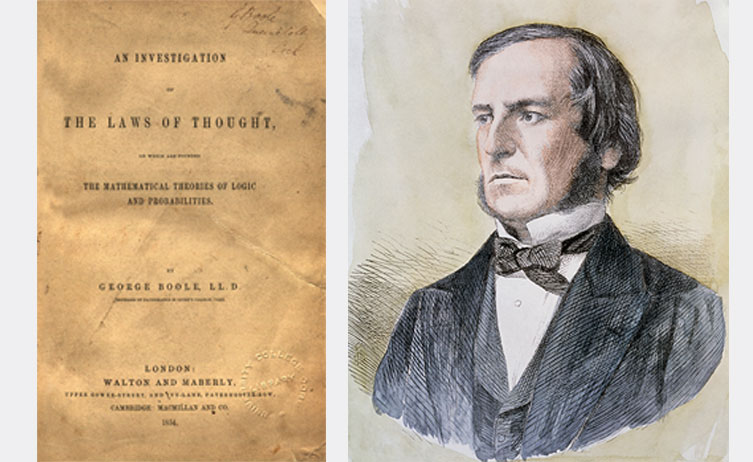
\includegraphics[width=0.5\textwidth]{images/images_intro/gboole.jpg}
    \caption{British logician and philosopher George Boole (1815--1864) next to his book \textit{The Laws of Thought} (1854), the oldest known record of the word ``interpretability''.}
    \label{fig:george-boole}
\end{figure}

What is remarkable is that the first recorded occurrence of ``interpretability'' was in the context of logic and computation. Boole asked: \textit{when can we meaningfully apply formal mathematical operations beyond the specific conditions under which we understand them?}
In Boole's era, the concern was whether logical operations like addition could be applied outside their original interpretable contexts—where symbols and their sum represent concepts that humans can understand (e.g., red + apples = red apples). Today, we face an analogous dilemma with machine learning algorithms: black-box programs like neural networks~\cite{perceptron}, which learn complex, unintelligible representations, are often deployed in contexts where computations should be understood by humans (e.g., in medicine~\cite{black-box2}). 

\begin{figure}[htbp]
    \centering
    \begin{subfigure}[b]{0.7\textwidth}
        \centering
        \begin{tikzpicture}[
            node distance=2.5cm,
            auto,
            thick,
            state/.style={circle, draw, fill=blue!20, minimum size=1.5cm, text centered},
            environment/.style={rectangle, draw, dashed, fill=blue!10, rounded corners, minimum width=4cm, minimum height=2cm, text centered},
            agent/.style={rectangle, draw, fill=orange!20, rounded corners, minimum width=2cm, minimum height=1.5cm, text centered},
            robot/.style={rectangle, draw, fill=black!20, rounded corners, minimum width=2cm, minimum height=1.5cm, text centered},
            ml/.style={circle, draw, fill=purple!20, minimum width=2cm, minimum height=1cm, text centered},
            decision_box/.style={rectangle, draw, dashed, fill=gray!10, minimum width=7.5cm, minimum height=3cm, text centered},
            arrow/.style={->, thick, bend left=15},
            arrow_decision/.style={->, dashed, bend left=15}
        ]
            
            % Decision Making Box
            \node[decision_box] (decision_box) at (0.3,3.4) {};
            \node at (0.3,4.5) {\small{Decision Making}};
            
            % Robot (AI)
            \node[robot] (robot) at (-2.1,3.2) {
                \begin{minipage}{1.5cm}
                    \centering
                    \includesvg[width=0.4cm]{images/images_intro/network-mapping-svgrepo-com.svg}\\
                    \small{Neural network}
                \end{minipage}
            };
            
            % Doctor
            \node[agent] (doctor) at (2.5,3.2) {
                \begin{minipage}{1.5cm}
                    \centering
                    \includesvg[width=0.4cm]{images/images_intro/doctor-with-stethoscope-svgrepo-com.svg}\\
                    \small{Doctor}
                \end{minipage}
            };
            
            % Machine Learning component
            \node[ml] (ml) at (-7,3) {
                \begin{minipage}{1.8cm}
                    \centering
                    \includesvg[width=0.4cm]{images/images_intro/gear-file-svgrepo-com.svg}\\
                    \small{Machine learning}
                \end{minipage}
            };
            
            % Environment (Patient)
            \node[environment] (environment) at (0,-0.5) {
                \begin{minipage}{2cm}
                    \centering
                    \includesvg[width=0.8cm]{images/images_intro/patient-4.svg}\\
                    \small{Cancer patient}
                \end{minipage}
            };
            
            % Arrows
            \draw[arrow] (environment) to[bend left=30] node[left] {
                \begin{minipage}{2cm}
                    \centering
                    \includesvg[width=0.5cm]{images/images_intro/patient-clipboard-svgrepo-com.svg}\\
                    \small{Updated health status}
                \end{minipage}
            } (robot);
            \draw[arrow_decision] (robot) to node[above] {\small{Recommends}} (doctor);
            \draw[arrow_decision, red] (doctor) to node[below] {\small{Cannot interpret}} (robot);
            
        \draw[arrow] (doctor) to[bend left=30] node[right] {
                \begin{minipage}{1.5cm}
                    \centering
                    \includesvg[width=0.5cm]{images/images_intro/syringe-svgrepo-com.svg}\\
                \small{Administer chemotherapy}
                \end{minipage}
            } (environment);
            
            % ML learning arrows
            \draw[arrow] (environment) to[bend left=40] node[left] {
                \begin{minipage}{2cm}
                    \centering
                    \includesvg[width=0.5cm]{images/images_intro/patient-clipboard-svgrepo-com.svg}\\
                    \small{Treatment outcomes}
                \end{minipage}
            } (ml);
            \draw[arrow] (ml) to[bend left=20] node[above] {
                \begin{minipage}{1.5cm}
                    \centering
                    \small{Updates program}
                \end{minipage}
            } (robot);
            
        \end{tikzpicture}
        \caption{Black-box approach using neural networks}
        \label{fig:cancer-treatment-sdm-ml}
    \end{subfigure}
    
    \vspace*{1cm}
    
    \begin{subfigure}[b]{0.7\textwidth}
        \centering
        \begin{tikzpicture}[
            node distance=2.5cm,
            auto,
            thick,
            state/.style={circle, draw, fill=blue!20, minimum size=1.5cm, text centered},
            environment/.style={rectangle, draw, dashed, fill=blue!10, rounded corners, minimum width=4cm, minimum height=2cm, text centered},
            agent/.style={rectangle, draw, fill=orange!20, rounded corners, minimum width=2cm, minimum height=1.5cm, text centered},
            robot/.style={rectangle, draw, fill=green!20, rounded corners, minimum width=2cm, minimum height=1.5cm, text centered},
            ml/.style={circle, draw, fill=purple!20, minimum width=2cm, minimum height=1cm, text centered},
            decision_box/.style={rectangle, draw, dashed, fill=gray!10, minimum width=7.5cm, minimum height=3cm, text centered},
            arrow/.style={->, thick, bend left=15},
            arrow_decision/.style={->, dashed, bend left=15}
        ]
            
            % Decision Making Box
            \node[decision_box] (decision_box) at (0.3,3.4) {};
            \node at (0.3,4.5) {\small{Decision Making}};
            
            % Robot (AI)
            \node[robot] (robot) at (-2.1,3.2) {
                \begin{minipage}{1.5cm}
                    \centering
                    \includesvg[width=0.4cm]{images/images_intro/decision-tree-svgrepo-com.svg}\\
                    \small{Decision tree}
                \end{minipage}
            };
            
            % Doctor
            \node[agent] (doctor) at (2.5,3.2) {
                \begin{minipage}{1.5cm}
                    \centering
                    \includesvg[width=0.4cm]{images/images_intro/doctor-with-stethoscope-svgrepo-com.svg}\\
                    \small{Doctor}
                \end{minipage}
            };
            
            % Machine Learning component
            \node[ml] (ml) at (-7,3) {
                \begin{minipage}{1.8cm}
                    \centering
                    \includesvg[width=0.4cm]{images/images_intro/gear-file-svgrepo-com.svg}\\
                    \small{Interpretable machine learning}
                \end{minipage}
            };
            
            % Environment (Patient)
            \node[environment] (environment) at (0,-0.5) {
                \begin{minipage}{2cm}
                    \centering
                    \includesvg[width=0.8cm]{images/images_intro/patient-4.svg}\\
                    \small{Cancer patient}
                \end{minipage}
            };
            
            % Arrows
            \draw[arrow] (environment) to[bend left=30] node[left] {
                \begin{minipage}{2cm}
                    \centering
                    \includesvg[width=0.5cm]{images/images_intro/patient-clipboard-svgrepo-com.svg}\\
                    \small{Updated health status}
                \end{minipage}
            } (robot);
            \draw[arrow_decision] (robot) to node[above] {\small{Recommends}} (doctor);
            \draw[arrow_decision, green] (doctor) to node[below] {\small{Can interpret}} (robot);
            
            \draw[arrow] (doctor) to[bend left=30] node[right] {
                \begin{minipage}{1.5cm}
                    \centering
                    \includesvg[width=0.5cm]{images/images_intro/syringe-svgrepo-com.svg}\\
                    \small{Administer chemotherapy}
                \end{minipage}
            } (environment);
            
            % ML learning arrows
            \draw[arrow] (environment) to[bend left=40] node[left] {
                \begin{minipage}{2cm}
                    \centering
                    \includesvg[width=0.5cm]{images/images_intro/patient-clipboard-svgrepo-com.svg}\\
                    \small{Treatment outcomes}
                \end{minipage}
            } (ml);
            \draw[arrow] (ml) to[bend left=20] node[above] {
                \begin{minipage}{1.5cm}
                    \centering
                    \small{Updates program}
                \end{minipage}
            } (robot);
            
        \end{tikzpicture}
        \caption{Interpretable approach using decision trees}
        \label{fig:cancer-treatment-comparison}
    \end{subfigure}
    \caption{Comparison of sequential decision making approaches in cancer treatment. Top: a black-box neural network approach where the doctor cannot interpret the AI's recommendations. Bottom: an interpretable decision tree approach where the doctor can understand and verify the AI's recommendations. Both systems learn from treatment outcomes to improve their recommendations over time.}
    \label{fig:cancer-treatment-comparison-combined}
\end{figure}

In figure~\ref{fig:cancer-treatment-sdm-ml}, we illustrate how existing machine learning algorithms \textit{could} be used in principle to help with cancer treatment. In truth, this should be prohibited without some kind of transparency in the program's recommendation: why did the program recommend such a dosage?
In figure~\ref{fig:cancer-treatment-comparison}, we illustrate how machine learning \textit{should} be used in practice. We would ideally want doctors to have access to computer programs that can recommend ``good'' treatments and whose recommendations are interpretable. 

The key challenge of doing research on interpretability is the lack of formalism; there is no \textit{formal} definition of what constitutes an interpretable computer program. Hence, unlike for performance objectives, which have well-defined optimization targets (e.g., maximizing accuracy in supervised learning or maximizing rewards over time in reinforcement learning), it is not clear how to design machine learning algorithms to maximize interpretability. 
Despite this lack of formalism, the necessity of deploying interpretable programs has sparked many works, which we present next.
\subsection{What are existing approaches for learning interpretable programs?}

In this section we follow sections 6 and 7 of \cite{glanois-survey} and section 5 of \cite{milani-survey}. 
Furthermore we now employ the term ``model'' to refer to ``programs'' to be consistent with the machine learning research conventions.
Models are essentially mappings from inputs to outputs that can be trained with machine learning algorithms while programs might designate other types of computations like sorting.

\begin{figure}[htbp]
    \centering
    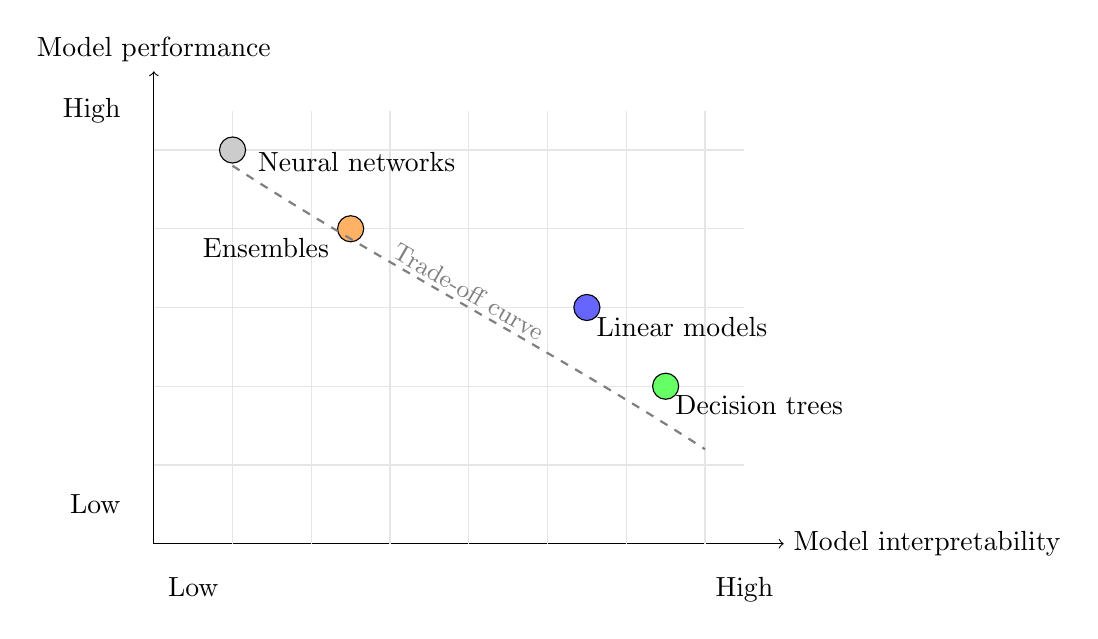
\begin{tikzpicture}
        % Define the axes
        \draw[->] (0,0) -- (8,0) node[right] {Model interpretability};
        \draw[->] (0,0) -- (0,6) node[above] {Model performance};
        
        % Add axis labels at the ends
        \node[below] at (0.5,-0.3) {Low};
        \node[below] at (7.5,-0.3) {High};
        \node[left] at (-0.3,0.5) {Low};
        \node[left] at (-0.3,5.5) {High};
        
        % Add grid lines (optional, subtle)
        \foreach \x in {1,2,...,7}
            \draw[gray!20] (\x,0) -- (\x,5.5);
        \foreach \y in {1,2,...,5}
            \draw[gray!20] (0,\y) -- (7.5,\y);
            
        % Position different model types
        % Deep Neural Networks (high performance, low interpretability)
        \node[circle, fill=black!20, draw, minimum size=8pt] at (1,5) {};
        \node[below right] at (1.2,5.1) {Neural networks};
        
        % Ensemble Methods (medium-high performance, low-medium interpretability)
        \node[circle, fill=orange!60, draw, minimum size=8pt] at (2.5,4) {};
        \node[below right] at (0.5,4) {Ensembles};
        
        % Linear Models (medium performance, high interpretability)
        \node[circle, fill=blue!60, draw, minimum size=8pt] at (5.5,3) {};
        \node[below right] at (5.5,3) {Linear models};
        
        % Decision Trees (medium-low performance, high interpretability)
        \node[circle, fill=green!60, draw, minimum size=8pt] at (6.5,2) {};
        \node[below right] at (6.5,2) {Decision trees};
        

        
        % Add a general trend line (optional)
        \draw[dashed, thick, gray] (1,4.8) .. controls (3,3.5) and (5,2.5) .. (7,1.2);
        \node[gray, rotate=-30] at (4,3.2) {\small Trade-off curve};
        
    \end{tikzpicture}
    \caption{The interpretability–performance trade-off in machine learning. Different model classes are positioned according to their typical interpretability and performance characteristics. The dashed line illustrates the general trade-off between these two properties.}
    \label{fig:interpretability-performance-tradeoff}
\end{figure}
Interpretable machine learning provides either local or global explanations \cite{glanois-survey}.
Global methods output a model whose outputs can be interpreted without additional computations, e.g., a decision tree~\cite{breiman1984classification}. By contrast, local methods require additional computations but are agnostic to the model class: they can give an \textit{approximate} interpretation of, e.g., neural network outputs.
In figure~\ref{fig:interpretability-performance-tradeoff} we present the popular trade-off between interpretability and performance of different model classes.

Given a model, LIME (Local Interpretable Model-agnostic Explanations)~\cite{lime} works by perturbing the input and learning a simple interpretable model locally to explain that particular prediction (see figure~\ref{fig:lime}). For each individual prediction, LIME provides explanations by identifying which features were most important for that specific decision.
Hence, as stated above, LIME needs to learn one local surrogate model per output to be interpreted; this requires substantial computation.

\begin{figure}
    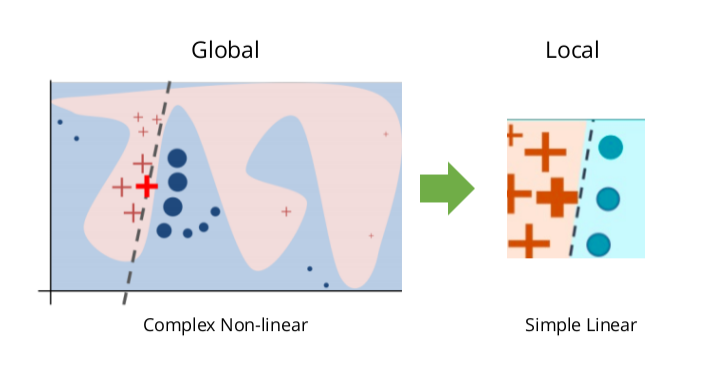
\includegraphics[width=0.9\textwidth]{images/lime.png}
    \caption{Local Interpretable Model-agnostic Explanations~\cite{lime} fit an interpretable linear model to data around the red cross prediction to be interpreted.}\label{fig:lime}
\end{figure}


\begin{figure}[htbp]
    \centering
    \begin{tikzpicture}[
        node distance=2cm,
        auto,
        thick,
        rl/.style={circle, draw, fill=purple!20, minimum width=1.5cm, minimum height=0.8cm, text centered},
        nn/.style={rectangle, draw, fill=black!20, rounded corners, minimum width=1.5cm, minimum height=1cm, text centered},
        sl/.style={circle, draw, fill=blue!20, minimum width=1.5cm, minimum height=0.8cm, text centered},
        dt/.style={rectangle, draw, fill=green!20, rounded corners, minimum width=1.5cm, minimum height=1cm, text centered},
        arrow/.style={->, thick},
        label/.style={font=\tiny, above},
        method_box/.style={rectangle, draw, dashed, minimum width=5cm, minimum height=3cm, text centered},
        method_box_indirect/.style={rectangle, draw, dashed, minimum width=9.5cm, minimum height=3cm, text centered}
    ]
        
        % Direct method box
        \node[method_box] (direct_box) at (-0.5,0) {};
        \node at (-0.5,1.7) {\small{Direct}};
        
        % Direct method - RL process
        \node[rl] (rl_direct) at (-2,0) {
            \begin{minipage}{1.2cm}
                \centering
                \includesvg[width=0.3cm]{images/images_intro/gear-file-svgrepo-com.svg}\\
                \tiny{Reinforcement learning}
            \end{minipage}
        };
        
        % Direct method - Decision Tree
        \node[dt] (dt_direct) at (1,0) {
            \begin{minipage}{1.2cm}
                \centering
                \includesvg[width=0.3cm]{images/images_intro/decision-tree-svgrepo-com.svg}\\
                \tiny{Decision tree}
            \end{minipage}
        };
        
        % Direct method arrow
        \draw[arrow] (rl_direct) -- (dt_direct) node[label, midway] {\tiny Learns};
        
        % Indirect method box
        \node[method_box_indirect] (indirect_box) at (7.1,0) {};
        \node at (6.8,1.7) {\small{Indirect}};
        
        % Indirect method - RL process
        \node[rl] (rl_indirect) at (3.5,0) {
            \begin{minipage}{1.2cm}
                \centering
                \includesvg[width=0.3cm]{images/images_intro/gear-file-svgrepo-com.svg}\\
                \tiny{Reinforcement learning}
            \end{minipage}
        };
        
        % Indirect method - Neural Network
        \node[nn] (nn_indirect) at (6,0) {
            \begin{minipage}{1.2cm}
                \centering
                \includesvg[width=0.3cm]{images/images_intro/network-mapping-svgrepo-com.svg}\\
                \tiny{Neural network}
            \end{minipage}
        };
        
        % Indirect method - Supervised Learning
        \node[sl] (sl_indirect) at (8.5,0) {
            \begin{minipage}{1.2cm}
                \centering
                \includesvg[width=0.3cm]{images/images_intro/gear-file-svgrepo-com.svg}\\
                \tiny{Supervised learning}
            \end{minipage}
        };
        
        % Indirect method - Decision Tree
        \node[dt] (dt_indirect) at (11,0) {
            \begin{minipage}{1.2cm}
                \centering
                \includesvg[width=0.3cm]{images/images_intro/decision-tree-svgrepo-com.svg}\\
                \tiny{Decision Tree}
            \end{minipage}
        };
        
        % Indirect method arrows
        \draw[arrow] (rl_indirect) -- (nn_indirect) node[label, midway] {\tiny Learns};
        \draw[arrow] (nn_indirect) -- (sl_indirect) node[label, midway] {\tiny Generates data};
        \draw[arrow] (sl_indirect) -- (dt_indirect) node[label, midway] {\tiny Learns};
        
    \end{tikzpicture}
    \caption{Comparison of direct and indirect approaches for learning interpretable models in sequential decision making}
    \label{fig:direct-vs-indirect-methods}
\end{figure}

Global approaches are either direct or indirect~\cite{milani-survey}. 
Direct algorithms, such as decision tree induction~\cite{breiman1984classification}, \textit{directly} learn an interpretable model optimizing some objective (see figure~\ref{fig:interpretability-performance-tradeoff}).
One key challenge motivating this thesis is that decision tree induction is well-developed for supervised learning but not for reinforcement learning.
To directly learn interpretable models for sequential decision making, one must design new algorithms which will be the core of the first part of this thesis. 

Most existing research has focused on developing indirect methods. 
Indirect methods for interpretable sequential decision making—sometimes called \textit{post hoc} methods—begin by learning a non-interpretable model (e.g., reinforcement learning of a neural network model), and then use supervised learning to fit an interpretable model that emulates the black-box.
This approach is called behavior cloning or imitation learning~\cite{behavior-cloning,dagger}, and many works on interpretable sequential decision rely on this indirect approach\cite{viper,PIRL}.
However we believe this might be problematic.

Indeed, unlike direct methods that return interpretable models optimizing the desired objective, indirect methods learn an interpretable model to match the behavior of a black-box that itself optimizes the objective of interest. 
Hence, there is no guarantee that optimizing this surrogate objective yields the best interpretability–performance trade-offs. 
figure~\ref{fig:direct-vs-indirect-methods} illustrates the key difference between these two approaches. 

Verifiable Reinforcement learning via Policy Extraction, or VIPER \cite{viper}, is a strong indirect method to learn decision tree models for sequential decision making. VIPER first trains a neural network model with reinforcement learning and then fit a decision tree to minimize the disagreement between the nerual network and the tree outputs given the same inputs.
They show that decision tree models, in addition to being transparent, are also fast to verify in the formal sense of the term \cite{maraboupy}.
Programmatic models are an interpretable class that contains decision trees. 
Programmatically Interpretable Reinforcement Learning (PIRL) \cite{PIRL} synthesizes programs in a domain-specific language, also by imitating a neural network model. 

Beyond direct and indirect learning, a complementary strategy is to train experts that are inherently easier to imitate and understand.
This is achieved by adding interpretability-oriented regularization during training. In~\cite{parbhoo}, authors regularize the neural netowk model during training such that indirect approaches will be biased towards more interpretable trees.

Beyond transparency and verifiability, interpretability also supports detecting specification or reward misalignment in sequential decision making: by exposing the decision process of a model, one can identify goal misspecification or unintended shortcuts.
Such shortcuts can be, for example, following the shadow of someone instead of actually following someone because for the model they lead to the same reactions.
The learning of interpretable models for misalignment detection has been heavily studied by Quentin Delfosse contemporarily to this manuscript \cite{scobots}\cite{shindo2024blendrl}\cite{nudge}\cite{ocatari}.

\textit{Interpretable} decision making constrains the model class so that the computation is transparent by construction. 
On the other hand, \textit{explainable} decision making, keeps black-box models and generates post hoc explanations of their decisions. 
Such explanations can take various forms: visual explanations with saliency maps \cite{Puri2020Explain}, attribution such as SHAP\cite{shap}, attention-based highlighting \cite{attention}.
Causal approaches learn explicit causal models to support contrastive reasoning \cite{madumal}.
While useful for insight, these explanations are often subjective and might not be faithful to the underlying computations~\cite{Atrey2020Exploratory}.
For safety-critical settings, this motivates our focus on models that are interpretable by design.
Next we describe technical preliminaries useful to understand the content of this manuscript.

\section{Technical preliminaries}

\subsection{What are decision trees?}\label{sec:dt}

As the reader might have already guessed, we will put great emphasis as decision tree models as a mean to study interpretability.
While other interpretable models might have other properties that the ones we will highlight through this thesis, one conjecture from \cite{glanois-survey} is that interpretable models are all hard to optimize or learn because they are non-differentiable in nature.
This something that will be key in our study of decision tree models that we introduce next and that we illustrate in figure~\ref{fig:dt}.

\begin{definition}[Decision tree]
    A decision tree is a rooted tree $T = (V, E)$ where:
    \begin{itemize}
    \item Each internal node $v \in V$ is associated with a test function $f_v: \mathcal{X} \rightarrow \{0, 1\}$ that maps input features $x \in \mathcal{X}$ to a Boolean.
    \item Each edge $e \in E$ from an internal node corresponds to an outcome of the associated test function.
    \item Each leaf node $\ell \in V$ is associated with a prediction $y_\ell \in \mathcal{Y}$, where $\mathcal{Y}$ is the output space.
    \item For any input $x \in \mathcal{X}$, the tree defines a unique path from root to leaf, determining the prediction $T(x) = y_\ell$ where $\ell$ is the reached leaf.
    \end{itemize}
    The depth of a tree is the maximum path lentght from root to any leaf.
    \end{definition}

\begin{figure}[htbp]
    \centering
    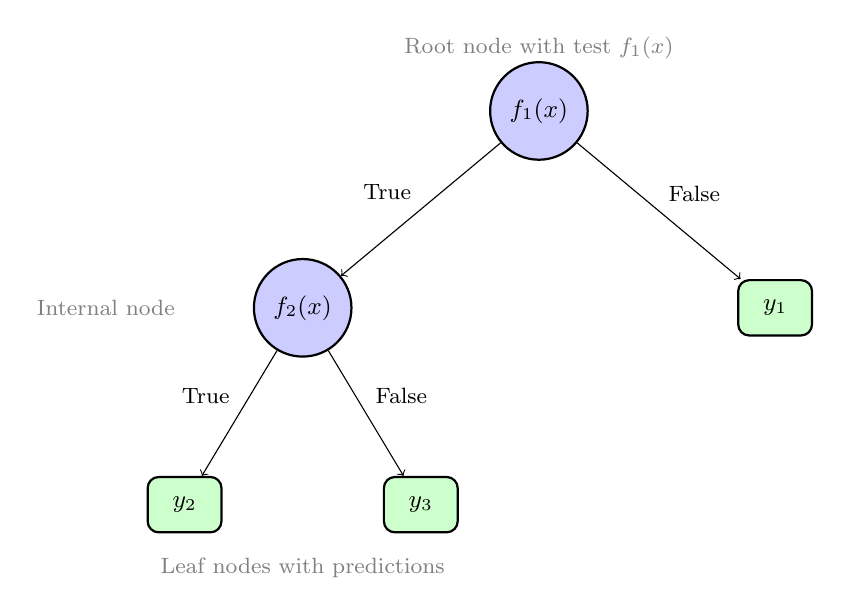
\begin{tikzpicture}[
        scale=1.0,
        decision/.style={circle, draw, thick, fill=blue!20, text width=2.5em, text centered, minimum height=2.5em, font=\small},
        leaf/.style={rectangle, draw, thick, fill=green!20, text width=2em, text centered, rounded corners, minimum height=2em, font=\small},
        edge_label/.style={font=\footnotesize, midway}
    ]
        % Root decision node
        \node[decision] (root) at (0,0) {$f_1(x)$};
        
        % Second level nodes
        \node[decision] (left_decision) at (-3, -2.5) {$f_2(x)$};
        \node[leaf] (right_leaf) at (3, -2.5) {$y_1$};
        
        % Third level nodes (leaves)
        \node[leaf] (left_left) at (-4.5, -5) {$y_2$};
        \node[leaf] (left_right) at (-1.5, -5) {$y_3$};
        
        % Connections with labels
        \draw[->] (root) -- (left_decision) node[edge_label, above left] {True};
        \draw[->] (root) -- (right_leaf) node[edge_label, above right] {False};
        \draw[->] (left_decision) -- (left_left) node[edge_label, above left] {True};
        \draw[->] (left_decision) -- (left_right) node[edge_label, above right] {False};
        
        % Add labels for components
        \node[font=\footnotesize, text=gray] at (0, 0.8) {Root node with test $f_1(x)$};
        \node[font=\footnotesize, text=gray] at (-5.5, -2.5) {Internal node};
        \node[font=\footnotesize, text=gray] at (-3, -5.8) {Leaf nodes with predictions};
        
    \end{tikzpicture}
    \caption{A generic depth 2 decision tree with 3 nodes and 3 leaves. Internal nodes contain test functions $f_v(x): \mathcal{X} \rightarrow \{0,1\}$ that map input features to boolean values. Edges represent the outcomes of these tests (True/False), and leaf nodes contain predictions $y_\ell \in \mathcal{Y}$. For any input $x$, the tree defines a unique path from root to leaf.}
    \label{fig:dt}
\end{figure}

\subsection{How to learn decision trees?}\label{sec:sl}
Training decision trees to optimize the supervised learning objective~\ref{def:sl} is well studied.

\begin{definition}[Supervised learning]\label{def:sl}
    Assume that we have access to a set of $N$ examples denoted $\mathcal{E} = {\{(x_i, y_i)\}}_{i=1}^N$. Each datum $x_i$ is described by a set of $p$ features. $y_i \in {\mathcal Y}$ is the label associated with $x_i$.
    For a classification task $\mathcal{Y}=\{1,\ldots,K\}$ and for a regression task $\mathcal{Y}\subseteq \mathbb{R}$.
    The goal of supervised learning is to find a classifier (or regressor) $f:X \rightarrow  y$ where $f$ is model in $\mathacal{F}$, e.g. neural networks or decision tres.
    \begin{align}
        f^* &= \underset{f \in \mathcal{F}}{\operatorname{argmin}}\ \frac{1}{N}\overset{N}{\underset{i=1}{\sum}}{\ell}(y_i, f(x_i)) + \alpha C(f),
        \label{eq:suplearning}
    \end{align}
    where $C: \mathcal{F} \rightarrow \mathbb{R}$ is a regularization penalty.
    \end{definition}

The Classification and Regression Trees (CART) algorithm \cite{breiman1984classification} (algorithm~\ref{alg:cart}), developed by Leo Breiman and colleagues (figure~\ref{fig:leo-breiman}), is one of the most widely used methods for learning decision trees from supervised data.
CART builds binary decision trees through a greedy, top-down approach that recursively partitions the feature space. 
At each internal node, the algorithm selects the feature and threshold that best splits the data according to a purity criterion such as the Gini impurity for classification or mean squared error for regression.
CART uses threshold-based test functions of the form $f_v(x) = \mathbb{I}[x[\text{feature}] \leq \text{threshold}]$, where $\mathbb{I}[\cdot]$ is the indicator function. 
The key idea is to find splits that maximize the homogeneity of the resulting subsets. 
We use CART as well as other decision tree algorithms in this manuscript and rely on the scikit-learn implementations \cite{scikit-learn} for our experiments.

In particular, in the second part we will challenge decision tree algorithms that perform better than CART for the supervised learning objective.
In the first and third parts, we study CART in conjunction with reinforcement learning as a means to obtain decision trees for sequential decision making.

In the next few sections we present the material related to sequential decision making.

\begin{figure}
    \centering
    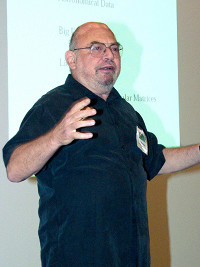
\includegraphics[width=0.3\textwidth]{images/images_intro/Leo_Breiman.jpg}
    \caption{The american statistician Leo Breiman (1928-2005) author of \textit{Classification and Regression Trees} (1984)}
    \label{fig:leo-breiman}
\end{figure}

\RestyleAlgo{ruled}
\SetKwComment{Comment}{}{}
\begin{algorithm}
    \KwData{Training data $(X, y)$ where $X \in \mathbb{R}^{n \times p}$ and $y \in \{1, 2, \ldots, K\}^n$}
    \KwResult{Decision tree $T$}
    
    \SetKwProg{Fn}{Function}{:}{}
    \SetKwFunction{BuildTree}{BuildTree}
    \SetKwFunction{BestSplit}{BestSplit}
    \SetKwFunction{Gini}{Gini}
    \SetKwFunction{MajorityClass}{MajorityClass}
    
    \Fn{\BuildTree{$X, y$}}{
        \If{stopping criterion met}{
            \Return leaf node with prediction MajorityClass$(y)$
        }
        
        $(feature, threshold) \leftarrow$ BestSplit$(X, y)$ \\
        
        \If{no valid split found}{
            \Return leaf node with prediction MajorityClass$(y)$
        }
        
        Split data: $X_{left}, y_{left} = \{(x_i, y_i) : x_i[feature] \leq threshold\}$ \\
        \hspace{2.5cm} $X_{right}, y_{right} = \{(x_i, y_i) : x_i[feature] > threshold\}$ \\
        
        $left\_child \leftarrow$ BuildTree$(X_{left}, y_{left})$ \\
        $right\_child \leftarrow$ BuildTree$(X_{right}, y_{right})$ \\
        
        \Return internal node with test function $f_v(x) = \mathbb{I}[x[feature] \leq threshold]$ and children $(left\_child, right\_child)$
    }
    
    \Fn{\BestSplit{$X, y$}}{
        $best\_gain \leftarrow 0$ \\
        $best\_feature \leftarrow None$ \\
        $best\_threshold \leftarrow None$ \\
        
        \For{each feature $f \in \{1, 2, \ldots, p\}$}{
            \For{each unique value $v$ in $X[:, f]$}{
                $y_{left} \leftarrow \{y_i : X[i, f] \leq v\}$ \\
                $y_{right} \leftarrow \{y_i : X[i, f] > v\}$ \\
                
                $gain \leftarrow$ Gini$(y) - \frac{|y_{left}|}{|y|}$Gini$(y_{left}) - \frac{|y_{right}|}{|y|}$Gini$(y_{right})$ \\
                
                \If{$gain > best\_gain$}{
                    $best\_gain \leftarrow gain$ \\
                    $best\_feature \leftarrow f$ \\
                    $best\_threshold \leftarrow v$ \\
                }
            }
        }
        \Return $(best\_feature, best\_threshold)$
    }
    
    \Fn{\Gini{$y$}}{
        \Return $1 - \sum_{k=1}^K \left(\frac{|\{i : y_i = k\}|}{|y|}\right)^2$ \Comment{// Gini impurity}
    }
    
    \Return BuildTree$(X, y)$
    \caption{CART for decision tree induction to optimize the supervised learning objective~\ref{def:sl}}\label{alg:cart}
\end{algorithm}

\subsection{Markov decision processes and problems}
\begin{figure}[htbp]
    \centering
    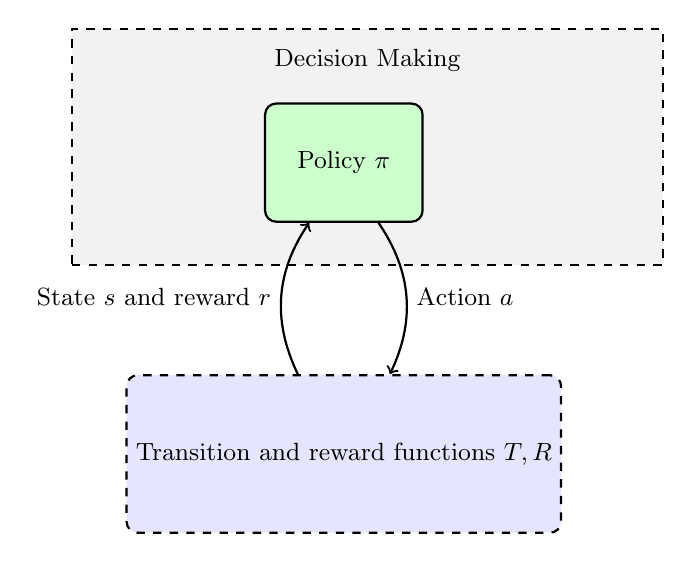
\begin{tikzpicture}[
        node distance=2.5cm,
        auto,
        thick,
        state/.style={circle, draw, fill=blue!20, minimum size=1.5cm, text centered},
        environment/.style={rectangle, draw, dashed, fill=blue!10, rounded corners, minimum width=4cm, minimum height=2cm, text centered},
        agent/.style={rectangle, draw, fill=orange!20, rounded corners, minimum width=2cm, minimum height=1.5cm, text centered},
        robot/.style={rectangle, draw, fill=green!20, rounded corners, minimum width=2cm, minimum height=1.5cm, text centered},
        decision_box/.style={rectangle, draw, dashed, fill=gray!10, minimum width=7.5cm, minimum height=3cm, text centered},
        arrow/.style={->, thick, bend left=15},
        arrow_decision/.style={->, dashed, bend left=15}
    ]
        
        % Decision Making Box
        \node[decision_box] (decision_box) at (0.3,3.4) {};
        \node at (0.3,4.5) {\small{Decision Making}};
        
        % Robot (AI)
        \node[robot] (robot) at (0,3.2) {\small{Policy $\pi$}};
        
        
        % Environment (Patient)
        \node[environment] (environment) at (0,-0.5) {\small{Transition and reward functions $T, R$}};
        
        % Arrows
        \draw[arrow] (environment) to[bend left=30] node[left] {\small{State $s$ and reward $r$}} (robot);
        \draw[arrow] (robot) to[bend left=30] node[right] {\small{Action $a$}} (environment);
        
    \end{tikzpicture}
    \caption{Markov decision process}
    \label{fig:MDP}
\end{figure}

Markov decision processes (MDPs) were first introduced in the 1950s by Richard Bellman~\cite{Bellman}.
Informally, an MDP models how an agent acts over time to achieve a goal. 
At every time step, the agent observes its current state (e.g., patient weight and tumor size) and takes an action (e.g., administers a certain amount of chemotherapy).
The agent receives a reward that helps evaluate the quality of the action with respect to the goal (e.g., tumor size decreases when the objective is to cure cancer).
Finally, the agent transitions to a new state (e.g., the updated patient state) and repeats this process over time. 
Following Martin L. Puterman's book on MDPs\cite{puterman}, we formally define:
\begin{definition}[Markov decision process]\label{def:mdp} An MDP is a tuple $\mathcal{M} = \langle S, A, R, T, T_0 \rangle$ where:
\begin{itemize}
\item $S$ is a finite set of states $s \in \mathbb{R}^n$ representing all possible configurations of the environment.
\item $A$ is a finite set of actions $a \in \mathbb{Z}^m$ available to the agent.
\item $R: S \times A \rightarrow \mathbb{R}$ is the reward function that assigns a real-valued reward to each state-action pair.
\item $T: S \times A \rightarrow \Delta(S)$ is the transition function that maps state-action pairs to probability distributions over next states, where $\Delta(S)$ denotes the probability simplex over $S$.
\item $T_0 \in \Delta(S)$ is the initial distribution over states.
\end{itemize}
\end{definition}

Informally, the goal of a model output actions given states is to behave so as to obtain as much reward as possible over time.
For example, in cancer treatment, the best outcome is to eliminate the patient's tumor as quickly as possible.
We can formally this goal as an optimization problem as follows.

\begin{definition}[Markov decision problem]\label{def:mdp-obj} Given an MDP $\mathcal{M}=\langle S, A, R, T, T_0 \rangle$ (~\ref{def:mdp}), the objective of a model, aslo known as a policy $\pi: S \rightarrow A$ is to maximize the expected discounted sum of rewards:
$$J(\pi) = \mathbb{E}\left[\sum_{t=0}^{\infty} \gamma^t R(s_t, a_t) \mid s_0 \sim T_0, a_t = \pi(s_t), s_{t+1} \sim T(s_t, a_t)\right]$$
where $\gamma \in (0,1]$ is the discount factor that controls the trade-off between immediate and future rewards.
\end{definition}

Hence, algorithms presented in this manuscript aim to find solutions to Markov decision problems, i.e., to model the optimal policy: $\pi^\star =\underset{\pi}{\operatorname{argmax}}J(\pi)$.
For the rest of this text, by abuse of notation, we denote both a Markov decision process and the associated Markov decision problem by MDP.

\subsection{Example: a grid-world MDP}
\begin{figure}[h]
    \centering
    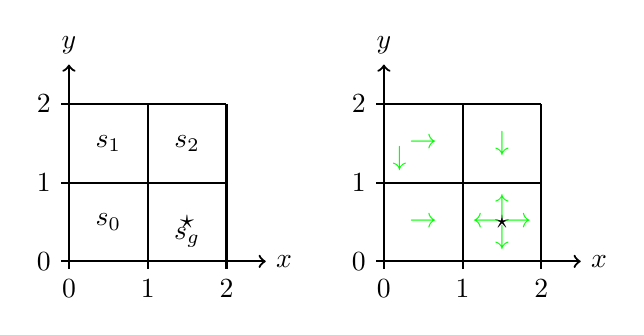
\begin{tikzpicture}
        \tikzstyle{grid}=[draw, thick, fill=gray!10]
        
        % Draw grid
        \draw[grid] (0,0) grid (2,2);
        
        % Add axes
        \draw[thick, ->] (0,0) -- (2.5,0) node[right] {$x$};
        \draw[thick, ->] (0,0) -- (0,2.5) node[above] {$y$};
        
        % Add tick marks and labels
        \foreach \x in {0,1,2} {
            \draw[thick] (\x,0) -- (\x,-0.1) node[below] {$\x$};
        }
        \foreach \y in {0,1,2} {
            \draw[thick] (0,\y) -- (-0.1,\y) node[left] {$\y$};
        }
        
        % Add state labels clockwise from bottom left
        \node at (0.5,0.5) {$s_0$};
        \node at (1.5,0.5) {$\star$};
        \node at (1.5,0.3) {$s_g$};
        \node at (1.5,1.5) {$s_2$};
        \node at (0.5,1.5) {$s_1$};


        % Draw grid
        \draw[grid] (4,0) grid (6,2);
        
        % Add axes
        \draw[thick, ->] (4,0) -- (6.5,0) node[right] {$x$};
        \draw[thick, ->] (4,0) -- (4,2.5) node[above] {$y$};
        
        % Add tick marks and labels
        \draw[thick] (4,0) -- (4,-0.1) node[below] {$0$};
        \draw[thick] (5,0) -- (5,-0.1) node[below] {$1$};
        \draw[thick] (6,0) -- (6,-0.1) node[below] {$2$};
        

        \foreach \y in {0,1,2} {
            \draw[thick] (4,\y) -- (3.9,\y) node[left] {$\y$};
        }
        
        % Add state labels clockwise from bottom left
        \node at (4.5,0.5) {{\color{green} $\rightarrow$}};
        \node at (5.5,0.5) {$\star$};
        \node at (5.5,0.7) {{\color{green} $\uparrow$}};
        \node at (5.5,0.3) {{\color{green} $\downarrow$}};
        \node at (5.7,0.5) {{\color{green} $\rightarrow$}};
        \node at (5.3,0.5) {{\color{green} $\leftarrow$}};
        \node at (5.5,1.5) {{\color{green} $\downarrow$}};
        \node at (4.2,1.3) {{\color{green} $\downarrow$}};
        \node at (4.5,1.5) {{\color{green} $\rightarrow$}};
    \end{tikzpicture}
    \caption{A grid-world MDP (left) and optimal actions w.r.t. the objective~\ref{def:mdp-obj} (right).}\label{example:grid}
    \end{figure}

In figure~\ref{example:grid}, we present a very simple MDP(~\ref{def:mdp}).
This MDP is essentially a grid where the starting state is chosen at random and the goal is to reach the bottom-right cell as fast as possible in order to maximize the objective~\ref{def:mdp-obj}.
The state space is discrete with state labels representing 2D-coordinates.
The actions are to move up, left, right, or down. The MDP transitions to the resulting cell. 
Only the bottom-right cell gives reward 1 and is an absorbing state, i.e., once in the state, the MDP stays in this state forever.
The optimal actions that get to the goal as fast as possible in every state (cell) are presented in green.

Next we present the tools to find solutions to MDPs and retrieve such optimal policies.

\subsection{Exact solutions for Markov decision problems}\label{sec:values}
It is possible to compute the exact optimal policy $\pi^\star$ using dynamic programming\cite{Bellman}.
Indeed, one can leverage the Markov property to find for all states the best action to take based on the reward of upcoming states.
\begin{definition}[Value of a state]\label{def:vs} 
    The value of a state $s\in S$ under policy $\pi$ is the expected discounted sum of rewards starting from state $s$ and following policy $\pi$:
    $$V^\pi(s) = \mathbb{E}\left[\sum_{t=0}^{\infty} \gamma^t R(s_t, a_t) \mid s_0 = s, a_t = \pi(s_t), s_{t+1} \sim T(s_t, a_t)\right]$$
    Applying the Markov property gives a recursive definition of the value of $s$ under policy $\pi$:
    $$V^\pi(s) = R(s,\pi(s)) + \gamma \sum_{s' \in S} T(s,\pi(s),s')\,V^\pi(s')$$
    where $T(s,a,s')$ is the probability of transitioning to state $s'$ when taking action $a$ in state $s$.
\end{definition}
\begin{definition}[Optimal value of a state] The optimal value of a state $s\in S$, $V^\star(s)$, is the value of state $s$ when following the optimal policy: $V^{\pi^{\star}}(s)$.
    $$V^{\star}(s) = V^{\pi^{\star}}(s) = \underset{\pi}{\max}\left[J(\pi)\right]$$
\end{definition}
\begin{definition}[Optimal value of a state–action pair] The optimal value of a state–action pair $(s,a)\in S\times A$, $Q^\star(s,a)$, is the value when taking action $a$ in state $s$ and then following the optimal policy.
    $$Q^{\star}(s,a) = R(s, a) + \gamma\sum_{s'\in S} T(s,a,s')\,V^{\star}(s')$$
\end{definition}

Hence, objective~\ref{def:mdp-obj}: $\pi^{\star} = \underset{\pi}{\operatorname{argmax}}\mathbb{E}\left[V^{\pi}(s_0)|s_0\sim T_0 \right]$.
The well-known Value Iteration algorithm~\ref{alg:value_iteration} solves this problem exactly. 

\RestyleAlgo{ruled}
\SetKwComment{Comment}{}{}
\begin{algorithm}
    \KwData{MDP $\mathcal{M} = \langle S, A, R, T, T_0 \rangle$, convergence threshold $\theta$}
    \KwResult{Optimal policy $\pi^*$}
    Initialize $V(s) = 0$ for all $s \in S$ \\
    \Repeat{$\Delta < \theta$}{
        $\Delta \leftarrow 0$ \\
        \For{each state $s \in S$}{
            $v \leftarrow V(s)$ \\
            $V(s) \leftarrow \max_a \left[ R(s,a) + \gamma \sum_{s' \in S} T(s,a,s') V(s') \right]$ \Comment{// Bellman optimality update}
            $\Delta \leftarrow \max(\Delta, |v - V(s)|)$
        }
    }
    \For{each state $s \in S$}{
        $\pi^*(s) \leftarrow \arg\max_a \left[ R(s,a) + \gamma \sum_{s' \in S} T(s,a,s') V(s') \right]$ \Comment{// Extract optimal policy}
    }
    \caption{Value Iteration}\label{alg:value_iteration}
\end{algorithm}

More realistically, neither the transition kernel $T$ nor the reward function $R$ of the MDP are known; e.g., the doctor cannot \textbf{know} how the tumor and the patient's health will change after a dose of chemotherapy, but can only \textbf{observe} the change.
This distinction in available information parallels the distinction between dynamic programming and reinforcement learning (RL), described next. 

\subsection{Reinforcement learning of approximate solutions to MDPs}\label{sec:rl}
\begin{figure}
    \centering
    \begin{subfigure}[b]{0.22\textwidth}
        \centering
        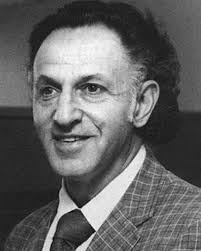
\includegraphics[width=0.7\textwidth]{images/images_intro/bellman.jpeg}
        \caption{R. Bellman}
    \end{subfigure}
    \hfill
    \begin{subfigure}[b]{0.22\textwidth}
        \centering
        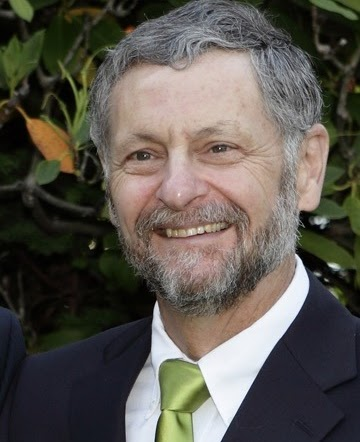
\includegraphics[width=0.7\textwidth]{images/images_intro/puterman.jpg}
        \caption{M.L. Puterman}
    \end{subfigure}
    \hfill
    \begin{subfigure}[b]{0.22\textwidth}
        \centering
        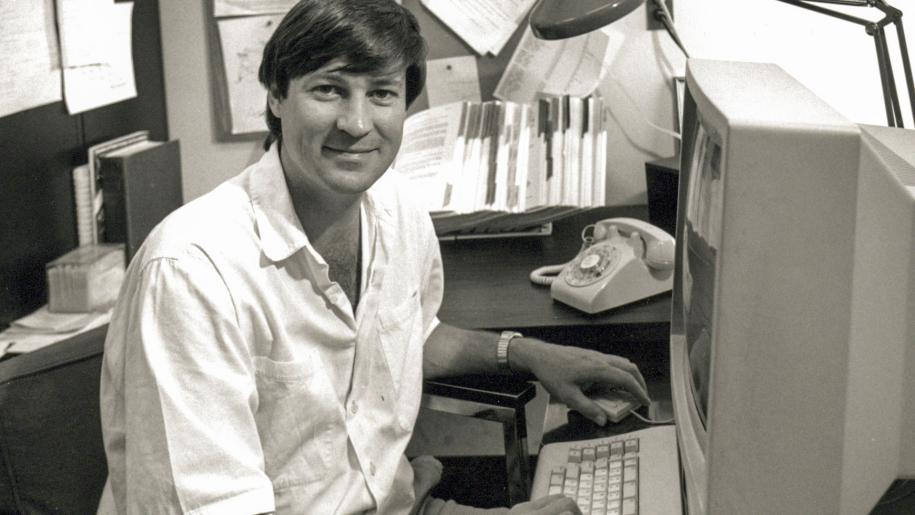
\includegraphics[width=1.2\textwidth]{images/images_intro/Barto_1982_umass_amherst.jpg}
        \caption{A. Barto}
    \end{subfigure}
    \hfill
    \begin{subfigure}[b]{0.22\textwidth}
        \centering
        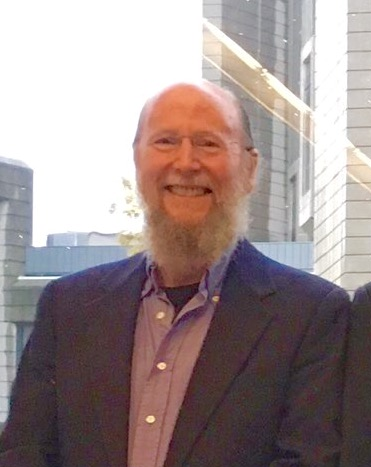
\includegraphics[width=0.67\textwidth]{images/images_intro/sutton.jpg}
        \caption{R. Sutton}
    \end{subfigure}
       \caption{The godfathers of sequential decision making. Andrew Barto and Richard Sutton are the ACM Turing Prize 2024 laureate and share an advisor advisee relationship.}
       \label{fig:rl-pioneers}
\end{figure}

Reinforcement learning algorithms popularized by Richard Sutton~\cite{sutton}(figure~\ref{fig:rl-pioneers}) don't \textbf{compute} an optimal policy but rather \textbf{learn} an approximate one based on sequences of observations ${(s_t, a_t, r_t, s_{t+1})}_t$.
RL algorithms usually fall into two categories: value-based (cite) and policy search~\cite{pg_sutton}.
Examples of these approaches are shown in algorithms~\ref{alg:qlearning},~\ref{alg:sarsa} and~\ref{alg:reinforce}.
Q-learning and Sarsa compute an approximation of $Q^{\star}$ using temporal difference learning. Q-learning is \textit{off policy}, it collects new transisitions with a random policy, e.g. epsilon-greedy, while Sarsa is on policy, it collects new transitions greedily w.r.t. the current q-values estimates.
Policy gradient algorithms leverages the policy gradient theorem to approximate $\pi^{\star}$.
The goal of an RL algorithm (also called agent) is to learn a policy that solves a Markov decision problem(~\ref{def:mdp-obj}) without access to transitions and rewards from the MDP.
From now on, we refer to~\ref{def:mdp-obj} as the RL objective.

Q-learning, Sarsa, and Policy gradients are known to converge to the optimal value or (locally) optimal policy under some conditions.
The books from Puterman~\cite{puterman}, or Sutton and Barto~\cite{sutton}, offer a great overview of MDPs and algorithms to solve them.
There are many other ways to learn policies such as simple random search~\cite{random-search} or model-based reinforcement learning~\cite{dyna}. 
However, not many algorithms consider the learning of policies that can be easily understood by humans which we discuss next and that is the core of this manuscript.

\RestyleAlgo{ruled}
\SetKwComment{Comment}{}{}
\begin{algorithm}
    \KwData{MDP $\mathcal{M} = \langle S, A, R, T, T_0 \rangle$, learning rate $\alpha$, exploration rate $\epsilon$}
    \KwResult{Policy $\pi$}
    Initialize $Q(s,a) = 0$ for all $s \in S, a \in A$ \\
    \For{each episode}{
        Initialize state $s_0 \sim T_0$ \\
        \For{each step $t$}{
            Choose action $a_t$ using $\epsilon$-greedy: $a_t = \arg\max_a Q(s_t,a)$ with prob. $1-\epsilon$ \\
            Take action $a_t$, observe $r_t = R(s_t,a_t)$ and $s_{t+1} \sim T(s_t,a_t)$ \\
            $Q(s_t,a_t) \leftarrow Q(s_t,a_t) + \alpha[r_t + \gamma \max_{a'} Q(s_{t+1},a') - Q(s_t,a_t)]$ \\
            $s_t \leftarrow s_{t+1}$ \\
        }
    }
    $\pi(s) = \arg\max_a Q(s,a)$ \Comment{// Extract greedy policy}
    \caption{Value-based RL (Q-Learning)}\label{alg:qlearning}
\end{algorithm}


\RestyleAlgo{ruled}
\SetKwComment{Comment}{}{}
\begin{algorithm}
    \KwData{MDP $\mathcal{M} = \langle S, A, R, T, T_0 \rangle$, learning rate $\alpha$, exploration rate $\epsilon$}
    \KwResult{Policy $\pi$}
    Initialize $Q(s,a) = 0$ for all $s \in S, a \in A$ \\
    \For{each episode}{
        Initialize state $s_0 \sim T_0$ \\
        Choose action $a_0$ using $\epsilon$-greedy: $a_0 = \arg\max_a Q(s_0,a)$ with prob. $1-\epsilon$ \\
        \For{each step $t$}{
            Take action $a_t$, observe $r_t = R(s_t,a_t)$ and $s_{t+1} \sim T(s_t,a_t)$ \\
            Choose action $a_{t+1}$ using $\epsilon$-greedy: $a_{t+1} = \arg\max_a Q(s_{t+1},a)$ with prob. $1-\epsilon$ \\
            $Q(s_t,a_t) \leftarrow Q(s_t,a_t) + \alpha[r_t + \gamma Q(s_{t+1},a_{t+1}) - Q(s_t,a_t)]$ \\
            $s_t \leftarrow s_{t+1}$ \\
            $a_t \leftarrow a_{t+1}$ \\
        }
    }
    $\pi(s) = \arg\max_a Q(s,a)$ \Comment{// Extract greedy policy}
    \caption{Value-based RL (Sarsa)}\label{alg:sarsa}
\end{algorithm}


\RestyleAlgo{ruled}
\SetKwComment{Comment}{}{}
\begin{algorithm}
    \KwData{MDP $\mathcal{M} = \langle S, A, R, T, T_0 \rangle$, learning rate $\alpha$, policy parameters $\theta$}
    \KwResult{Policy $\pi_\theta$}
    Initialize policy parameters $\theta$ \\
    \For{each episode}{
        Generate trajectory $\tau = (s_0, a_0, r_0, s_1, a_1, r_1, \ldots)$ following $\pi_\theta$ \\
        \For{each time step $t$ in trajectory}{
            $G_t \leftarrow \sum_{k=t}^{T} \gamma^{k-t} r_k$ \Comment{// Compute return}
            $\theta \leftarrow \theta + \alpha G_t \nabla_\theta \log \pi_\theta(a_t|s_t)$ \Comment{// Policy gradient update}
        }
    }
    \caption{Policy Gradient RL (REINFORCE)}\label{alg:reinforce}
\end{algorithm}


\section{Deep reinforcement learning for large or continuous state spaces}\label{sec:drl}

Reinforcement learning has also been successfully combined with function approximations \cite{td-gammon} to solve MDPs with large discrete state spaces or continuous state spaces ($S \subset \mathbb{R^n}$).
Such continuous states MDP can be formalized as factored MDPs\cite{fmdp}:

\begin{definition}[Factored Markov decision process] A factored MDP is an MDP\cite{def:mdp} where the state space is a hyperrectangle: $S\subseteq \mathbb{R}^n$.
\end{definition}

From now on, all the MDPs we study in the this manuscript are factored unless stated otherwise. 
We also consider that the Example MDP(\ref{example:grid}) is continuous with two state dimensions.
In the rest of this manuscript, unless stated otherwise, we write $\boldsymbol{s}$ a state vector in a continuous space.
Note that discrete states MDP can be encoded into factored MDP by one-hot encoding individual states.

Deep Q-Networks (DQN)~\cite{dqn}, described in algorithm~\ref{alg:dqn} was a breakthrough in modern reinforcement learning.
Authors successfully extended the Q-learning (algorithm~\ref{alg:qlearning}) to the function approximation setting by introduction target networks to mitigate distributional shift in the td error and replay buffer to increase sample efficiency (see figure~\ref{fig:dqn} for the tricks used to adap Q-learning to the function approximation setting).
DQN achieved super-human performance on a set of Atari games.

Proximal Policy Optimization (PPO)~\cite{ppo}, described in algorithm~\ref{alg:ppo}, is an actor-critic algorithm\cite{pg_sutton} optimizing neural network policies. 
Actor-critic algorithms are instances of policy gradient algorithms where the cumulative discounted rewards--the returns--are also estimated with a neural network. 
Actor-critic are not as simple efficient as DQN but is known to work well in a variety of domains including robot control in simulation among others.

\begin{algorithm}
    \KwData{MDP $\mathcal{M} = \langle S, A, R, T, T_0 \rangle$, learning rate $\alpha$, exploration rate $\epsilon$, Q-network parameters $\theta$, update frequency $C$}
    \KwResult{Policy $\pi$}
    Initialize Q-network parameters $\theta$ and target network parameters $\theta^- = \theta$ \\
    Initialize replay buffer $\mathcal{B} = \emptyset$ \\
    \For{each episode}{
        Initialize state $s_0 \sim T_0$ \\
        \For{each step $t$}{
            Choose action $a_t$ using $\epsilon$-greedy: $a_t = \arg\max_a Q_\theta(\boldsymbol{s}_t,a)$ with prob. $1-\epsilon$ \\
            Take action $a_t$, observe $r_t = R(s_t,a_t)$ and $\boldsymbol{s}_{t+1} \sim T(\boldsymbol{s}_t,a_t)$ \\
            Store transition $(\boldsymbol{s}_t, a_t, r_t, \boldsymbol{s}_{t+1})$ in $\mathcal{B}$ \\
            Sample random batch $(\boldsymbol{s}_i, a_i, r_i, \boldsymbol{s}_{i+1}) \sim \mathcal{B}$ \\
            $y_i = r_i + \gamma \max_{a'} Q_{\theta^-}(\boldsymbol{s}_{i+1}, a')$ \Comment{// Compute target}
            $\theta \leftarrow \theta - \alpha \nabla_\theta (Q_\theta(\boldsymbol{s}_i, a_i) - y_i)^2$ \Comment{// Update Q-network}
            \If{$t \bmod C = 0$}{
                $\theta^- \leftarrow \theta$ \Comment{// Update target network}
            }
            $\boldsymbol{s}_t \leftarrow \boldsymbol{s}_{t+1}$ \\
        }
    }
    $\pi(\boldsymbol{s}) = \arg\max_a Q_\theta(\boldsymbol{s},a)$ \Comment{// Extract greedy policy}
    \caption{Deep Q-Network (DQN)}\label{alg:dqn}
\end{algorithm}

\begin{figure}
    \centering
    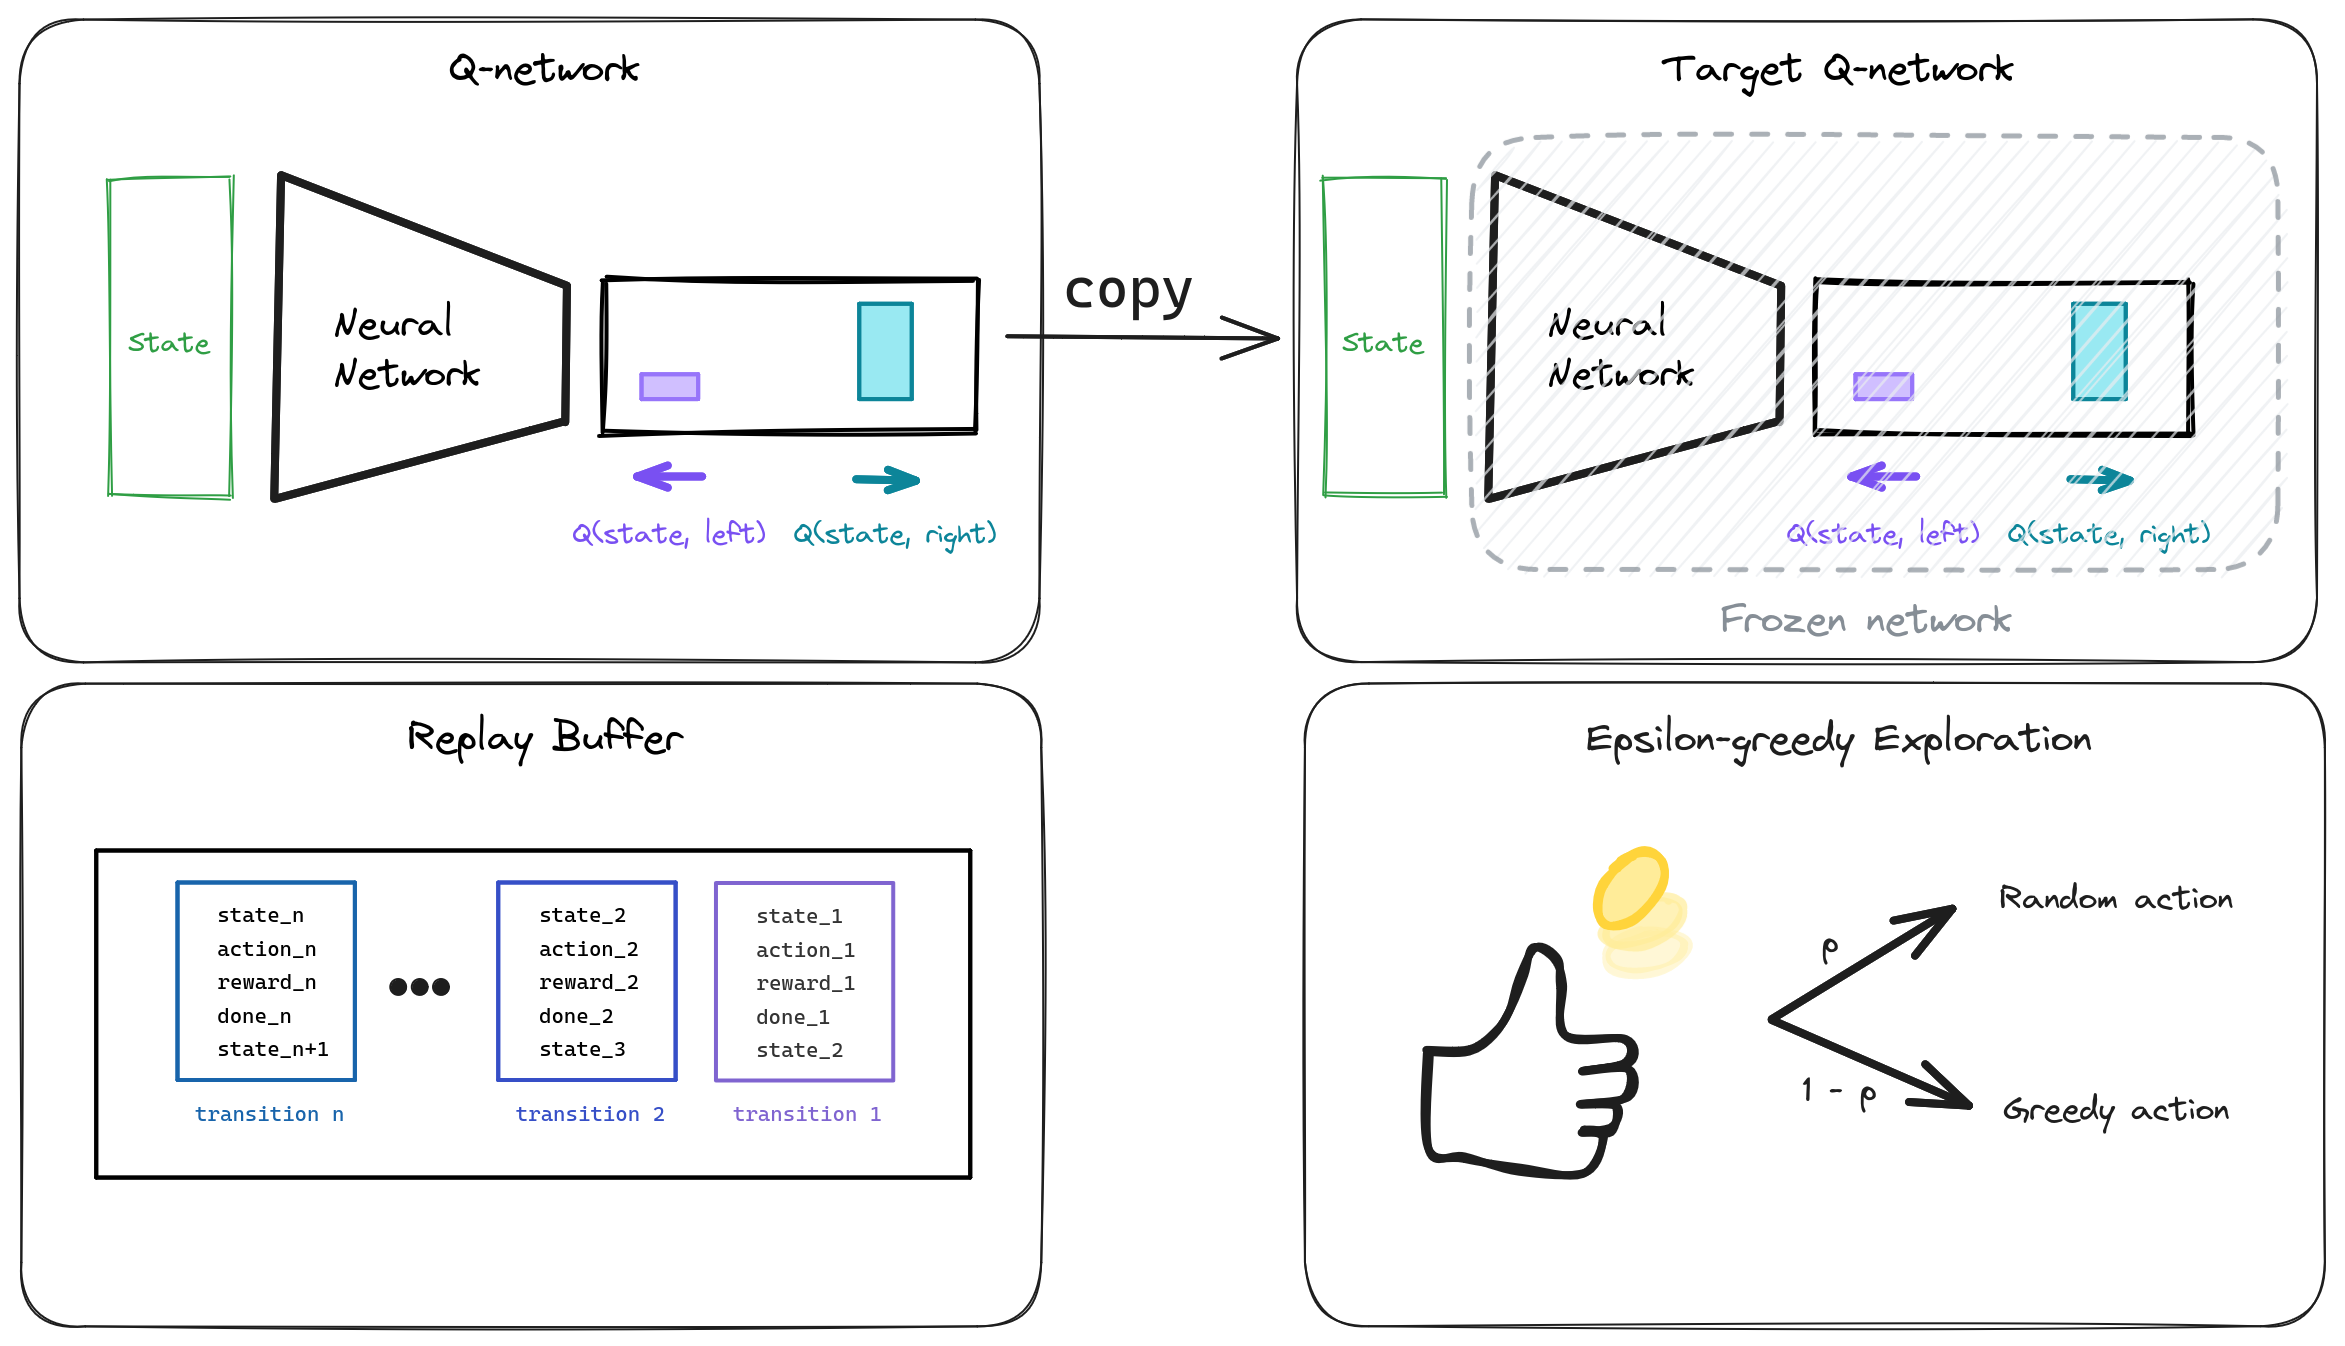
\includegraphics[width=1\textwidth]{images/dqn_schema.png}
    \caption{DQN tricks added to the vanilla Q-learning (algorithm~\ref{alg:qlearning}). Courtesy of Antonin Raffin.}
\end{figure}


\begin{algorithm}
    \KwData{MDP $\mathcal{M} = \langle S, A, R, T, T_0 \rangle$, learning rate $\alpha$, policy parameters $\theta$, clipping parameter $\epsilon$, value function parameters $\phi$}
    \KwResult{Policy $\pi_\theta$}
    Initialize policy parameters $\theta$ and value function parameters $\phi$ \\
    \For{each episode}{
        Generate trajectory $\tau = (\boldsymbol{s}_0, a_0, r_0, \boldsymbol{s}_1, a_1, r_1, \ldots)$ following $\pi_\theta$ \\
        \For{each time step $t$ in trajectory}{
            $G_t \leftarrow \sum_{k=t}^{T} \gamma^{k-t} r_k$ \Comment{// Compute return}
            $A_t \leftarrow G_t - V_\phi(\boldsymbol{s}_t)$ \Comment{// Compute advantage}
            $r_t(\theta) \leftarrow \frac{\pi_\theta(a_t|\boldsymbol{s}_t)}{\pi_{\theta_{old}}(a_t|\boldsymbol{s}_t)}$ \Comment{// Compute probability ratio}
            $L^{CLIP}_t \leftarrow \min(r_t(\theta) A_t, \text{clip}(r_t(\theta), 1-\epsilon, 1+\epsilon) A_t)$ \Comment{// Clipped objective}
            $\theta \leftarrow \theta + \alpha \nabla_\theta L^{CLIP}_t$ \Comment{// Policy update}
            $\phi \leftarrow \phi + \alpha \nabla_\phi (G_t - V_\phi(\boldsymbol{s}_t))^2$ \Comment{// Value function update}
        }
        $\theta_{old} \leftarrow \theta$ \Comment{// Update old policy}
    }
    \caption{Proximal Policy Optimization (PPO)}\label{alg:ppo}
\end{algorithm}
In this manuscript we study those two deep reinforcement learning algorithms for various problems and use their stable-baselines3 implementations\cite{stable-baselines3}.

\subsection{Imitation learning: a baseline (indirect) interpretable reinforcement learning method}\label{sec:imit}

Unlike PPO or DQN for neural networks, there does not exist an algorithm that trains decision tree policies to optimize the RL objective (\ref{def:mdp-obj}).
In fact, we will show in the first part of the manuscript that training decision trees that optimize the RL objective is very difficult.

Hence, many interpretable reinforcement learning approaches first train a neural network policy with, e.g., DQN or PPO to optimize the RL objective (\ref{def:mdp-obj}), and then fit, e.g., a decision tree using CART (algorithm\ref{alg:cart}) to optimize the supervised learning objective (\ref{def:sl}) with the neural policy's actions as targets.
This approach is known as imitation learning and is essentially training a policy to optimize the objective:

\begin{definition}[Imitation learning]\label{def:il}
Given an MDP $\mathcal{M}$ (\ref{def:mdp}) expert policy $\pi^*$ and a policy class $\Pi$, the imitation learning objective is to find a policy $\pi \in \Pi$ that minimizes the expected action disagreement with the expert:
\begin{equation}
\min_{\pi \in \Pi} \mathbb{E}_{\boldsymbol{s} \sim \rho(\boldsymbol{s})} \left[ \mathcal{L}(\pi(\boldsymbol{s}), \pi^*(\boldsymbol{s})) \right]
\end{equation}
where $\rho(\boldsymbol{s})$ is the state distribution in $\mathcal{M}$ induced by the expert policy and $\mathcal{L}$ is a loss function measuring the disagreement between the learned policy's action $\pi(s)$ and the expert's action $\pi^*(s)$.
\end{definition}

There are two main imitation learning methods used for interpretable reinforcement learning.
Dagger (\cite{PIRL}; algorithm~\ref{alg:dagger}) is a straightforward way to fit a decision tree policy to optimize the imitation learning objective\ref{def:il}.
VIPER (\cite{viper}; algorithm~\ref{alg:viper}) was designed specifically for interpretable reinforcement learning.
VIPER reweights the transitions collected by the neural network expert by a function of the state–action value\ref{sec:values}.
The authors of VIPER showed that decision tree policies fitted with VIPER tend to have the same RL objective value as Dagger trees while being more interpretable (shallower or with fewer nodes) and sometimes outperform Dagger trees.
Dagger and VIPER are two strong baselines for decision tree learning in MDPs, but they optimize a surrogate objective only, even though in practice the resulting decision tree policies often achieve high RL objective value.

We use the two algorithms extensively throughout the manuscript.

Next we show how to learn a decision tree policy for the Example MDP \ref{example:grid}.
\begin{algorithm}
    \caption{Dagger\cite{dagger}}\label{alg:dagger}
    \KwIn{Expert policy $\pi^*$, MDP $M$, policy class $\Pi$}
    \KwOut{Fitted student policy $\hat{\pi}_i$}
    
    % Initialize empty dataset and initial policy
    Initialize dataset $\mathcal{D} \gets \emptyset$\;
    Initialize $\hat{\pi}_1$ arbitrarily from $\Pi$\;
    
    \For{$i \gets 1$ \KwTo $N$}{
        % Create mixed policy using expert and current policy
        \lIf{i = 1}{
        $\hat{\pi} \gets \pi^*$\
        }
          \lElse{
            $\pi_i \gets \hat{\pi}_i$
          } \label{alg:expert-or-student}
        % Collect data using mixed policy
        Sample transitions from $M$ using $\hat{\pi}$\;
        % Get expert actions for visited states
        Collect dataset $\mathcal{D}_i \gets \{ (\boldsymbol{s}, \pi^*(\boldsymbol{s})) \}$ of states visited by $\hat{\pi}$\;
        
        % Aggregate datasets
        $\mathcal{D} \gets \mathcal{D} \cup \mathcal{D}_i$\;
        
        % Train new policy
       Fit classifier/regressor $\hat{\pi}_{i+1}$ on $\mathcal{D}$\;\label{alg:fit}
    }
    \Return $\hat{\pi}$\;
    \end{algorithm}


    \begin{algorithm}
        \caption{VIPER\cite{viper}}\label{alg:viper}
        \KwIn{Expert policy $\pi^*$, Expert Q-function $Q^*$, MDP $M$, policy class $\Pi$}
        \KwOut{Fitted student policy $\hat{\pi}_i$}
        
        % Initialize empty dataset and initial policy
        Initialize dataset $\mathcal{D} \gets \emptyset$\;
        Initialize $\hat{\pi}_1$ arbitrarily from $\Pi$\;
        
        \For{$i \gets 1$ \KwTo $N$}{
            % Create mixed policy using expert and current policy
            \lIf{i = 1}{
            $\hat{\pi} \gets \pi^*$\
            }
              \lElse{
                $\pi_i \gets \hat{\pi}_i$
              } \label{alg:expert-or-student}
            % Collect data using mixed policy
            Sample transitions from $M$ using $\hat{\pi}$\;
            % Get expert actions for visited states
            Weight each transition by $w(\boldsymbol{s}) \gets V^{\pi^*}(\boldsymbol{s}) - \min_a Q^{\pi^*}(\boldsymbol{s}, a)$\;
            Collect dataset $\mathcal{D}_i \gets \{ (\boldsymbol{s}, \pi^*(\boldsymbol{s}), w(\boldsymbol{s})) \}$ of states visited by $\hat{\pi}$\;            
            % Aggregate datasets
            $\mathcal{D} \gets \mathcal{D} \cup \mathcal{D}_i$\;
            
            % Train new policy
           Fit classifier/regressor $\hat{\pi}_{i+1}$ on the weighted dataset $\mathcal{D}$\;\label{alg:fit}
        }
        \Return $\hat{\pi}$\;
        \end{algorithm}

\section{Your first decision tree policy}\label{sec:limits-il}
Now the reader should know how to train decision tree classifiers or regressors for supervised learning using CART\ref{sec:sl}.
The reader should also know what an MDP is and how to compute or learn policies that optimize the RL objective \ref{def:mdp-obj} with (deep) reinforcement learning\ref{sec:drl}.
Finally, the reader should now know how to obtain a decision tree policy for an MDP through imitation learning by first using RL to get an expert policy and then fitting decision trees to optimize the supervised learning objective\ref{def:sl}, using the expert's actions as labels.
Note that, in theory, there is no guarantee that such decision tree policies also maximize the RL objective; they optimize only the imitation learning objective\ref{def:il}.

In this section we present the first decision tree policies of this manuscript obtained using Dagger or VIPER after learning an expert policy and expert Q-function for the grid-world MDP \ref{example:grid} with Q-learning\ref{alg:qlearning}.
Recall the optimal policies for the grid-world, taking the green actions in each state in figure\ref{example:grid}. 
Among the optimal policies, the ones that take action to go left or up in the goal state can be problematic for imitation learning algorithms.

Indeed, we know that for this grid-world MDP there exists a decision tree policy that is optimal and very interpretable (depth-1): go right if the $x$-label of the state is greater than 1 and go left otherwise.
This tree takes exactly the same actions in the same states as some of the optimal policy from figure\ref{example:grid}.

In figure\ref{fig:trees-intro}, we present a depth-1 decision tree policy that is optimal w.r.t. the RL objective and a depth-1 tree that is suboptimal.
Indeed, figure\ref{fig:objectives} shows that the optimal depth-1 tree achieves exactly the same RL objective value as the optimal policies from figure\ref{example:grid}, independently of the discount factor $\gamma$.

Now a fair question is: can Dagger or VIPER retrieve such an optimal depth-1 tree given access to an expert optimal policy from figure\ref{example:grid}?

We start by running the standard Q-learning algorithm as presented in algorithm\ref{alg:qlearning} with $\epsilon=0.3$, $\alpha=0.1$ over 10,000 time steps.
The careful reader might wonder how ties are broken in the $\operatorname{argmax}$ operation from algorithm\ref{alg:qlearning}.
While Sutton and Barto break ties by index value in their book\cite{sutton} (the greedy action is the $\argmax$ action with smallest index), we show that the choice of tie-breaking greatly influences the performance of subsequent imitation learning algorithms.
Indeed, depending on how actions are ordered in practice, Q-learning may be biased toward some optimal policies rather than others.
While this does not matter for one who just wants to find an optimal policy, in our example of finding the optimal depth-1 decision tree policy, it matters \textit{a lot}.

In the left plot of figure\ref{fig:ql-il}, we see that Q-learning, independently of how ties are broken, consistently converges to an optimal policy over 100 runs (random seeds).
However, in the right plot of figure\ref{fig:ql-il}, where we plot the proportion over 100 runs of optimal decision trees returned by Dagger or VIPER at different stages of Q-learning, we observe that imitating the optimal policy obtained by breaking ties at random consistently yields more optimal trees than breaking ties by indices.
What actually happens is that the most likely output of Q-learning when ties are broken by indices is the optimal policy that goes left in the goal state,
which cannot be perfectly represented by a depth-1 decision tree, because there are three different actions taken and a binary tree of depth $D=1$ can only map to $2^D=2$ labels.

Despite this negative result, we still find that VIPER almost always finds the optimal depth-1 decision tree policy in terms of the RL objective\ref{def:mdp-obj} when ties are broken at random.
Importantly, this sheds light on the sub-optimality of indirect imitation w.r.t the RL objective (~\ref{def:mdp-obj}) and motivates the study of direct approaches.
\begin{figure}[h]
    \centering
    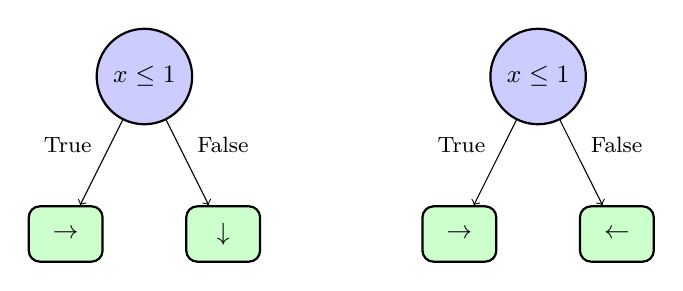
\begin{tikzpicture}[
        decision/.style={circle, draw, thick, fill=blue!20, text width=2.5em, text centered, minimum height=2.5em, font=\small},
        leaf/.style={rectangle, draw, thick, fill=green!20, text width=2em, text centered, rounded corners, minimum height=2em, font=\small},
        edge_label/.style={font=\footnotesize, midway}
    ]
        % Tree 4: if x <= 0.5 move right else move left
        \node[decision] (tree4_root) at (10,2) {$x \leq 1$};
        \node[leaf] (tree4_right) at (9,0) {$\rightarrow$};
        \node[leaf] (tree4_left) at (11,0) {$\leftarrow$};
        \draw[->] (tree4_root) -- (tree4_right) node[edge_label, above left] {True};
        \draw[->] (tree4_root) -- (tree4_left) node[edge_label, above right] {False};
        \tikzstyle{grid}=[draw, thick, fill=gray!10]


        % Tree 4: if x <= 0.5 move right else move left
        \node[decision] (tree5_root) at (5,2) {$x \leq 1$};
        \node[leaf] (tree5_right) at (4,0) {$\rightarrow$};
        \node[leaf] (tree5_left) at (6,0) {$\downarrow$};
        \draw[->] (tree5_root) -- (tree5_right) node[edge_label, above left] {True};
        \draw[->] (tree5_root) -- (tree5_left) node[edge_label, above right] {False};
        \tikzstyle{grid}=[draw, thick, fill=gray!10]

    \end{tikzpicture}
    \caption{Left, a sub-optimal depth-1 decision tree policy. On the right, an optimal depth-1 decision tree policy.}\label{fig:trees-intro}
    \end{figure}

\begin{figure}
    \centering
    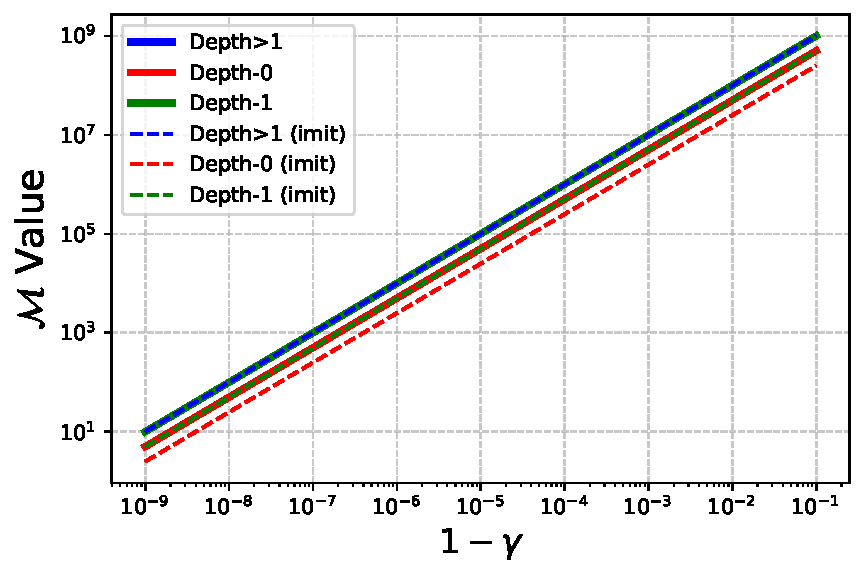
\includegraphics[width=0.6\textwidth]{images/images_part1/policy_values_comparison.pdf}
    \caption{The objective (\ref{def:mdp-obj}) values of the optimal policies from figure~\ref{example:grid} and of the decision tree policies from figure~\ref{fig:trees-intro}.}\label{fig:objectives}
\end{figure}

\begin{figure}
    \centering
    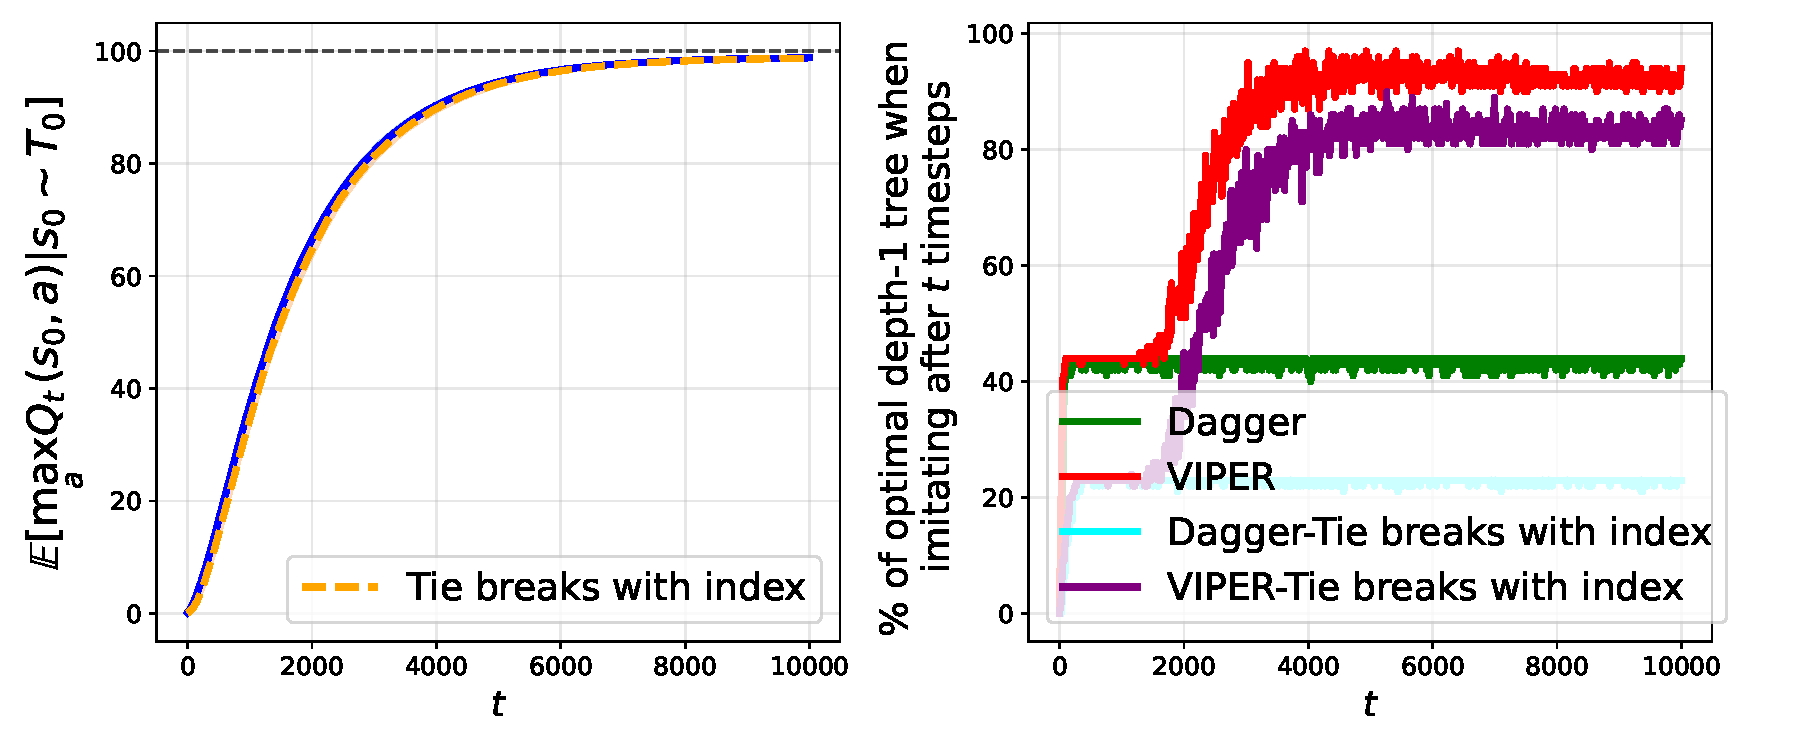
\includegraphics[width=1\textwidth]{images/images_part1/base_mdp.pdf}
    \caption{Left, sample complexity curve of Q-learning with default hyperparameters on the $2\times 2$ grid-world MDP over 100 random seeds. Right, performance of indirect interpretable methods when imitating the greedy policy with a tree at different Q-learning stages.}\label{fig:ql-il}
\end{figure}

Now that the reader has seen how to get an interpretable policy for an MDP, we believe it is ready to dive into the contributions of this thesis.

\section{Outline of the thesis}
Throughout our thesis, we make the assumption that constraing models (e.g. policies or classifiers) to decision trees is engouh ensuring interpretability.
In this thesis we study different decision tree learning algorithms in different settings. 
In the first part of the manuscript, we show that direct decision tree learning methods~\ref{fig:direct-vs-indirect-methods} struggle to find decision tree policies even for very simple sequential decision making problems.
For that, we first reproduce the work from\cite{topin2021iterative} that presents a formalism for learning decision tree policies that optimize~\ref{def:mdp-obj} directly using reinforcement learning, and then make connexions with hardness results from the partially observable MDPs (POMDPs)\cite{POMDP,chap2} litterature.
We defer the introduction of POMDPs to later sections.
In the second part of the manuscript, we formulate decision tree induction for supervised learning as solving a sequential decision making problem.
By formalizing decision tree induction for objective\ref{def:sl} as solving an MDP~\ref{def:mdp}, we design novel algorithms that achieve very good performances.

In the last part of the text, we lift our assumption about decision tree learning guaranteeing interpretability and study other model classes.
In particular, we leverage the simplicity of \textit{indirect} methods~\ref{fig:direct-vs-indirect} to imitate neural network experts with models from~\ref{fig:interpretability-performance-tradeoff} and and perform a large-scale empirical study of the interpretability-performances trade-offs on various sequential decision making tasks.
In Table~\ref{tab:summary-parts} we summarize the outline of this manuscript in terms of learning objective (~\ref{def:sl},~\ref{def:mdp-obj}, or~\ref{def:il}) and model class (figure~\ref{fig:interpretability-performance-tradeoff}).

\begin{table}[htbp]
    \centering
    \begin{tabular}{|l|c|c|c|c|}
        \hline
         & \textbf{Decision Trees} & \textbf{Linear} & \textbf{Ensembles} & \textbf{Neural Networks} \\
        \hline
        Supervised Learning & Part II &  & Part II & Part II\\
        \hline
        Reinforcement Learning & Part I, III & Part III & & Part I, III \\
        \hline
        Imitation Learning & Part I, III & Part III & & Part III \\
        \hline
    \end{tabular}
    \caption{Summary of objectives and model classes studied in this manuscript.}
    \label{tab:summary-parts}
\end{table}

We summarize our results as follows:

\begin{enumerate}
    \item Direct reinforcement learning of decision tree policies is hard because it involves POMDPs.
    \item One can use dynamic programming in MDPs to induce highly performing decision tree classifiers and regressors.
    \item In practice, controlling MDPs with interpretable policies does not necessarily decrease performances.
\end{enumerate}

% \begin{figure}[htbp]
%     \centering
%     \begin{tikzpicture}[
%         bubble/.style={rectangle, rounded corners=15pt, draw, thick, fill=blue!20, text width=3.5cm, text centered, minimum height=1.5cm, font=\small},
%         arrow/.style={->, thick},
%         label/.style={font=\footnotesize, text width=3cm, text centered}
%     ]
        
%         % Define the three vertices of the triangle
%         % Top bubble - chapter 1
%         \node[bubble] (ch1) at (0,4) {Part 1\\Direct learning of interpretable policies for MDPs};
        
%         % Bottom left bubble - chapter 2  
%         \node[bubble] (ch2) at (-4,0) {Part 2\\Supervised learning of decision tree classifiers with MDPs};
        
%         % Bottom right bubble - chapter 3
%         \node[bubble] (ch3) at (4,0) {Part 3\\Indirect learning of interpretable policies to compare different model classes};
        
%         % Arrow from chapter 1 to chapter 2
%         \draw[arrow] (ch1.south west) -- (ch2.north);
%         \node[label] at (-4.5,2.5) {Too difficult, let us assume uniform transitions};
        
%         % Arrow from chapter 1 to chapter 3  
%         \draw[arrow] (ch1.south east) -- (ch3.north);
%         \node[label] at (4.5,2.5) {Too difficult, let us use indirect approach};

%         % Arrow from chapter 1 to chapter 3  
%         \draw[arrow] (ch2.east) -- (ch3.west);
%         \node[label] at (0,1.1) {Use new decision tree induction to learn better interpretable policies};
        
        
%     \end{tikzpicture}
%     \caption{Thesis structure showing the progression from direct reinforcement learning of decision tree policies (chapter 1) to simplified approaches: supervised learning with uniform transitions (chapter 2) and indirect learning methods (chapter 3).}
%     \label{fig:thesis-outline}
% \end{figure}